\documentclass[11pt]{article}
\usepackage{acl2014}
\usepackage{times}
\usepackage{url}
\usepackage{latexsym}
\usepackage{graphicx}

\usepackage{amsmath}
\usepackage{amsfonts}
\usepackage{amssymb}

\title{Inside Outside Recursive Neural Network: A Unified Framework for 
Compositional Semantics and Meaning in Context}
\author{Phong Le, Remko Scha \textnormal{and} Willem Zuidema}

\begin{document}

\maketitle

\begin{abstract}
Although compositional semantics and meaning in context have a strong relation, 
it is surprising that there are no attempts tackling both. In this paper, we
propose a novel framework, Inside Outside Recursive Neural Network, 
which is able to compute phrase representations and context representations, 
thus solving the both challenges. Center to our framework is a new hypothesis that, 
according to our experimental results, is promising to lead to efficient unsupervised learning 
schemes for neural compositional semantics. 

\end{abstract}

%%%%%%%%%%%%%%%%%%%%%%%%%%%%%%%%%%%%%%%%%%
\section{Introduction}
\label{section introduction}

The reader should not have any problems to understand \textit{this} sentence although 
(s)he has never seen it. This is evidence that natural languages are compositional.
In order to capture this phenomenon, compositional semantics which relies on the principle 
of compositionality \emph{``The meaning of a whole is a function of the meanings of the parts 
and of the way they are syntactically combined''} \cite{partee_lexical_1995}
was introduced. Research on compositional semantics therefore focuses on two problems
(1) how to learn word representations, and (2) how to learn compositionality functions.

Phrase/word meaning in context, on the other hand, is about how meaning of a phrase/word
is changed by effect of it contexts. For instance, at the word level, the word `bank' in 
the two following constituents has different meanings
\begin{enumerate}
	\item along the east \textit{bank} of the river
	\item some big institutions, including \textit{banks}
\end{enumerate}
At the phrase level, depending on its context, a phrase should be understood literally or 
figuratively. %; e.g.,
%\begin{enumerate}
%	\item xyz
%	\item uvw
%\end{enumerate}

It is not difficult to realize that compositional semantics and meaning in context 
have a strong relation. To meaning in context, compositionality is helpful to compute 
context representations. In addition, if the target is a phrase, compositionality is 
essential for computing its meaning. To compositional semantics, context can be 
used to disambiguate word senses, thus lead to more reliable composition.
However, it is surprising that there are no attempts tackling both problems\footnote{
The work of \newcite{mitchell_vector-based_2008} is often considered 
as tackling both problems. However, to our opinion, their work is only for 
compositional semantics since comparing the meaning of a sentence (e.g, 
``The fire glowed'') to the meaning of a word (e.g., ``burned'') is an improper way 
to tackle meaning in context: the semantic similarity is not clear to be between
``the fire'' and ``burned'' or ``glowed'' and ``burned''.}.

In this paper, we propose a new framework, namely Inside Outside Recursive 
Neural Network (IORNN). IORNN is able to compute phrase representations 
as well as context representations, thus tackles the both challenges at the same time
in a unified framework.



%%%%%%%%%%%%%%%%%%%%%%%%%%%%%%%%%%%%%%%%%%

\section{Background}
\label{section background}

\subsection{Compositional Semantics}

Formal semantics, which uses formal languages to represent constituents, 
is the first attempt and well fits the principle of compositionality \cite{montague1970english}.
It firstly assumes that 
words are represented by lambda expressions, e.g. $\text{``John'' :- } \lambda x.john(x)$,
$\text{``walks'' :- } \lambda P \lambda y. walks(y) \wedge P(y)$. Then, using  
the lambda beta reduction rule as the compositionality function, it easily  
computes the meaning of a constituent ($\text{``John walks'' :- }
\lambda y. john(y) \wedge walks(y)$). 
This approach, although being sound with human beings and having a simple but 
powerful compositionality function, is very 
challenging to computers since automatically learning word representations 
is a difficult task \cite{DBLP:conf/coling/LeZ12}. 
%\cite{DBLP:conf/coling/LeZ12} propose a new approach, named
%Dependency-based Semantic Composition using Graphs (DeSCoG) to balance the difficulty 
%between lexical learning and compositionality, 
In addition, the fact that formal semantics only supports the truth values (True and False) 
and ignores lexical semantics restricts it to a short list of applications.

At the other extreme, distributional semantics, based on 
the distributional hypothesis \cite{lenci_distributional_2008}
\emph{``The degree of semantic similarity between two linguistic expressions A and B is a function
of the similarity of the linguistic contexts in which A and B can appear''},
is widely used for learning word meanings, which are represented in vector spaces.
That is because it has strong support from not only linguistics but
also cognitive science \cite{lenci_distributional_2008}. In addition, word representations 
can be learnt 
from unannotated data, which are redundant and free on the Internet, thanks to 
the flourish of unsupervised learning techniques, such as  latent semantic analysis 
\cite{landauer1998introduction}, neural network 
language model \cite{collobert_natural_2011,huang2012improving}, Brown clustering
algorithm \cite{brown1992class}, and 
spectral learning \cite{dhillon2012two}. And after all, due to the fact that it supports 
semantic similarity, distributional semantics has a wide range of applications: 
information retrieval, sentiment analysis, machine translation, etc. 
The distributional hypothesis, however, is not able to apply to phrasal semantics 
because of the sparsity of data: the number of phrases is 
infinite whereas available data is finite.

The most visible approach to tackle compositional semantics problem is to combine 
formal semantics and distributional semantics: the former for compositionality, the 
latter for word representations \cite{garrette2012formal}. It turns out this is 
not trivial since the two kinds of semantics have very different forms of representations
so that how to combine these forms is itself a difficult problem.

Another approach, which has been intensively studied recently, is distributional 
compositional semantics: 
if $\overrightarrow{a}, \overrightarrow{b}$ are vectors representing the meanings of 
the two items $a,b$, then the meaning vector $\overrightarrow{ab}$ of their constituent $ab$, 
yielded by the grammar rule $R$, is computed by \cite{mitchell_vector-based_2008}
\begin{equation}
\label{equation: general composition}
    \overrightarrow{ab} = f(\overrightarrow{a}, \overrightarrow{b}, R, K)
\end{equation}
where $f$ is a compositionality function and $K$ is background knowledge.
Many approaches were proposed to learn compositionality functions $f$. 
The most simple one is to use vector addition and multiplication as compositionality functions
\cite{mitchell_vector-based_2008}. 
%Those functions, although no parameters need to be optimized, 
%are too simple to capture real compositionality. 

Socher and colleagues propose two neural network frameworks: recursive auto encoder (RAE) 
\cite{socher_semi-supervised_2011} for 
unsupervised learning, and recursive neural network (RNN) for supervised learning with task-based 
training signal \cite{socher_learning_2010}
(e.g., for sentiment analysis, the training signal is the sentiments given by voters). 
The key idea of the RAE framework is: a compositionality function is a compression function, 
such that an input is able to be recovered from the output by a decompression function. 

\newcite{baroni_frege_2012}, \newcite{grefenstette_multi-step_2013} and others attempt the challenge 
in a different way. 
They use tensors to represent functor words (i.e., verbs, adjectives, etc.), 
linear maps as compositionality functions, and use contexts of phrases (in a similar way as in
distributional lexical semantics) for estimating tensors' elements and 
functions' parameters. 

Our work has some common points with the two approaches above. Similarly to the work of 
Socher and colleagues, IORNN uses recursive network architecture to construct 
phrase representations, but different in that it also constructs context representations and 
is trained in a very different manner. The training has the same key idea with the works of 
\newcite{baroni_frege_2012}, \newcite{grefenstette_multi-step_2013}: context is used 
as training signal. However, we only use contexts of words and thus avoid 
the sparsity of data.


\subsection{Meaning in Context}
\label{subsection meaning in context}
[TODO...]


%%%%%%%%%%%%%%%%%%%%%%%%%%%%%%%%%%%%%%%%%%
\section{Research Questions}
\label{section question}

First of all, we ask ourselves ``Which evidence is strong enough to be used for 
learning compositional semantics?'' %TODO: why not RAE, tensor...???
To answer this, we rely on the 
following observation: a human being can guess the meaning of an unknown 
word by making use of the meaning of its context. In other words, he computes 
(in his brain) the meaning of the context and then uses it to predict the meaning 
of the target unknown word (by setting some constraints to narrow down a list of 
possible meanings). Hence, if he correctly predicts the meaning of the unknown word, 
we can, at some degree of belief, say that he comprehends the meaning of the context. 
This idea is then captured in the following hypothesis
\begin{quote}
\textit{Hypothesis 1:} The agreement between words and contexts provides evidence for unsupervised 
compositional semantics learning. 
\end{quote}

Then, there are three questions need to be answered in order to implement the 
hypothesis
\begin{enumerate}
	\item How to construct phrase representations?
	\item How to construct context representations?
	\item How to use the agreement between words and 
	their contexts to learn compositionality functions?
\end{enumerate}
We present our answers in the next section.

%%%%%%%%%%%%%%%%%%%%%%%%%%%%%%%%%%%%%%%%%%

\section{Methodology}
\label{section methodology}
\subsection{Recursive Neural Network (RNN)}
\label{subsection rnn}
\newcite{socher_learning_2010} answer the first question ``How to construct phrase representations?'' 
by Recursive Neural Network (RNN) architecture. 
In order to see how RNN works, 
let's consider the following example. Assuming that there is a constituent with parse
tree $(p_2 \; (p_1 \; x \; y) \; z)$ (Figure~\ref{figure rnn}), and $\mathbf{x},\mathbf{y},\mathbf{z} \in \mathbb{R}^{n \times 1}$
are respectively the meanings of the three words $x$, $y$ and $z$. 
We will use a neural network 
which contains a weight matrix $\mathbf{W}_1  \in \mathbb{R}^{n \times n}$ for left children and 
a weight matrix $\mathbf{W}_2  \in \mathbb{R}^{n \times n}$ for right children 
to compute parents in a bottom up manner. Firstly, we use this network 
to compute $p_1$'s meaning
\begin{equation}
	\mathbf{p}_1 = f(\mathbf{W}_1 \mathbf{x} + \mathbf{W}_2 \mathbf{y} + \mathbf{b})
\end{equation}
where $\mathbf{b}$ is a bias vector, $f$ is an activation function (e.g. \textit{tanh} or \textit{logistic}).
Then, we use the same network to compute $p_2$'s meaning
\begin{equation}
	\mathbf{p}_2 = f(\mathbf{W}_1 \mathbf{p}_1 + \mathbf{W}_2 \mathbf{z} + \mathbf{b})
\end{equation}
This process is continued until we reach the root node.  This network is trained by 
a gradient-based optimization method (e.g., gradient descent) where the gradient 
over parameters is efficiently computed thanks to the backpropagation through structure
\cite{goller_learning_1996}. Using this architecture 
(and its extensions), Socher and colleagues successfully reach 
state-of-the-art results in syntactic parsing \cite{socher2013parsing} and 
sentiment analysis \cite{socher2013recursive}. 
\begin{figure}[h!]
	\center
	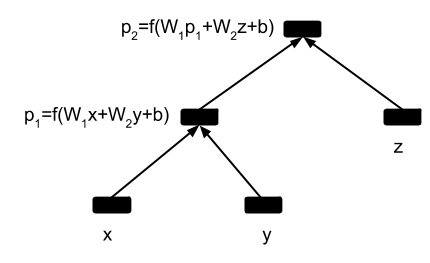
\includegraphics[scale=0.5]{RNN.png}
	\caption{Recursive Neural Network (RNN).}
	\label{figure rnn}
\end{figure}

In order to use this architecture in an unsupervised learning manner, 
\newcite{socher2011semi} replace the neural network in RNN by an autoencoder 
(and hence the new architecture is called Recursive Autoencoder - RAE), 
which is a feedforward neural network trained by forcing output equal to 
input (see Figure~\ref{figure rae}). Training a RAE is therefore to minmize 
the sum of reconstruction errors 
(i.e., $\|[\mathbf{x}';\mathbf{y}'] - [\mathbf{x};\mathbf{y}]\|^2$) at all internall nodes. 

\begin{figure}[h!]
	\center
	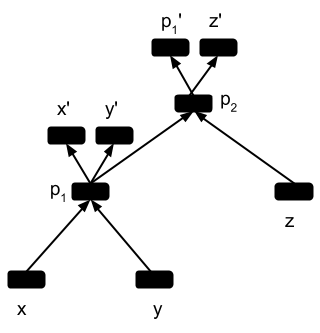
\includegraphics[scale=0.5]{RAE.png}
	\caption{Recursive Autoencoder (RAE).}
	\label{figure rae}
\end{figure}

%%%%%%%%%%%%%%%%%%%%%%%%%%%%%%%%%%%%%%%%%%

\subsection{Inside Outside Recursive Neural Network (IORNN)}
\label{subsection nlm}

None of the above architectures, RAE or RNN, compute contex representations. 
However, they give us a hint to do that. In this section, we will answer the second 
question ``How to construct context representations?'' by a new neural network 
architecture, namely Inside Outside Recursive Neural Network (IORNN). We also 
present this architecture by using the same example of constituent and parse tree 
$(p_2 \; (p_1 \; x \; y) \; z)$ (see Figure~\ref{figure iornn}).

\begin{figure}[h!]
	\center
	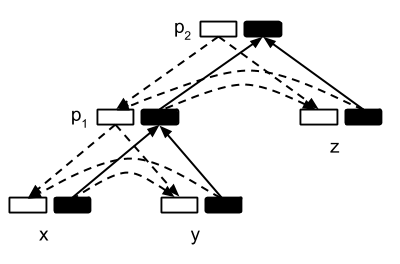
\includegraphics[scale=0.5]{IORNN.png}
	\caption{Inside-Outside Recursive Neural Network (IORNN). 
	Black rectangles correspond to inner meanings, 
	white rectangles correspond to outer meanings.}
	\label{figure iornn}
\end{figure}


Each node $u$ is assigned two vectors $\mathbf{o}_u$ and $\mathbf{i}_u$. The first one,
called \textit{outer meaning}, denotes the meaning of the context; the second one, 
called \textit{inner meaning}, denotes the meaning of the phrase that the node covers.

\paragraph{Word embeddings} (e.g., $\mathbf{i}_x$)
Similar to \newcite{socher_learning_2010,collobert_natural_2011}, given a string of binary
representations of words $(a, b, ..., w)$ (i.e., all of the entries of $w$ are zero except the one 
corresponding to the index of the word in the vocabulary), 
we first compute a string of vectors $(\mathbf{i}_{a},...,\mathbf{i}_{w})$ 
representing inner meanings of those words by using 
a look-up table (i.e., word embeddings) $\mathbf{L} \in \mathbb{R}^{n \times |V|}$, 
where $|V|$ is the size of the vocabulary and $n$ is the dimensionality of the vectors. 
This look-up table $\mathbf{L}$ could be seen as a storage of word meanings where each column 
is a vector representation of a word. Hence, 
\begin{equation}
    \label{equation compute word vector}
    \mathbf{i}_{w} = \mathbf{L} w \in \mathbb{R}^{n \times 1}
\end{equation}

\paragraph{Computing inner meaning} The inner meaning of a non-terminal node, say $p_1$, is given by
\begin{equation}
	\mathbf{i}_{p_1} = f(\mathbf{W}_1^i \mathbf{i}_{x} + \mathbf{W}_2^i \mathbf{i}_{y} + \mathbf{b}^i)
	\label{equation inner}
\end{equation}
where $\mathbf{W}_1^i, \mathbf{W}_2^i$ are $n \times n$ real matrices, 
$\mathbf{b}^i$ is a bias vector, and $f$ is an activation function, e.g. $tanh$. 
Intuitively, the inner meaning of a parent node is the function of the inner meanings 
of its children. This is similar to RNN.

\paragraph{Computing outer meaning} Because we process sentences individually, there is no information 
about discourse context. Therefore, the outer meaning of the root node, $\mathbf{o}_{root}$, is set to $\mathbf{o}_{\emptyset}$
, which is randomly initialized and then learnt later. 
To a node which is not the root, say $p_1$, the outer meaning is given by
\begin{equation}
	\mathbf{o}_{p_1} = g(\mathbf{W}_1^o \mathbf{o}_{p_2} + \mathbf{W}_2^o \mathbf{i}_{z} + \mathbf{b}^o)
	\label{equation outer}
\end{equation}
where $\mathbf{W}_1^o, \mathbf{W}_2^o$ are $n \times n$ real matrices, 
$\mathbf{b}^o$ is a bias vector, and $g$ is an activation function. 
Informally speaking, the outer meaning of a node (i.e., the meaning of 
its context) is the function of the outer meaning of its parent and the inner meaning 
of its sister. 

The reader could recognize the similarity between 
Equation~\ref{equation inner}, ~\ref{equation outer}
and the inside, outside probabilities given a parse tree.
That is why we name the architecture Inside-Outside Recursive Neural Network.

%%%%%%%%%%%%%%%%%%%%%%%%%%%%%%%%%%%%%%%%%%

\subsection{Training IORNN}
\label{subsection train iornn}

This section is to answer the final question ``How to use words and their contexts to 
learn compositionality functions?''. 

According to Hypothesis 1, there must be a strong correlation 
between $\mathbf{o}_{w}$ and $\mathbf{i}_{w}$ where $w$ is any word in 
a given sentence. The simplest way to train the network is to force 
$\mathbf{o}_{w_j} = \mathbf{i}_{w_j}$; hence, learning is to minimize the following 
loss function
\begin{equation}
	J(\theta) = \sum_{s \in D} \sum_{w \in s} \| \mathbf{o}_{w} - \mathbf{i}_{w} \|
\end{equation}
where $D$ is a set of training sentences and $\theta$ are the network parameters. 
However, that could be problematic because 
the meaning of context is not necessary the meaning of the target word.

Here, based on the observation that the meaning of context sets constraints on 
selecting a word to fill in the blank, one could suggest put a \textit{softmax} neuron 
unit on the top of each $\mathbf{o}_w$ in order to compute the probability $P(x|\mathbf{o}_w)$. 
Unfortunately, as pointed out by \newcite{collobert_natural_2011}, it might not work. 

Using the same method proposed by \newcite{collobert_natural_2011}, we train the network 
such that it gives to the correct target word a score higher than scores given to other words
by a margin of 1. 
The score $s(x,\mathbf{o}_w)$ given to a candidate word $x$ for a specific context 
$\mathbf{o}_w$ is computed by 
\begin{equation}
	u(x,\mathbf{o}_w) = f(\mathbf{W}^u_1 \mathbf{o}_w + \mathbf{W}^u_2 \mathbf{i}_x + \mathbf{b}^u) 
\end{equation}
\begin{equation}
	\label{equation score}
	s(x,\mathbf{o}_w) = \mathbf{W}^s u(x,\mathbf{o}_w) + \mathbf{b}^s
\end{equation}
where $\mathbf{W}_1^u,\mathbf{W}_2^u$ are $n \times k$ real matrices, $ \mathbf{W}^s$ is 
a $k \times 1$ matrix, and $\mathbf{b}^u, \mathbf{b}^s$ are bias vectors. (We fix $k=2n$.) 
Now, the objective function is the ranking criterion with respect to $\theta$
\begin{equation}
	J(\theta) = \sum_{s \in D} \sum_{w \in s} \sum_{x \in V} \max \{0, 1 - s(w,\mathbf{o}_w) + s(x,\mathbf{o}_w) \}
\end{equation}

To minimize the above objective function, we randomly pick up a word 
in the vocabulary as a corrupt example, then compute the gradient by the 
backpropagation through structure \cite{goller_learning_1996}. 
Following \newcite{socher2013recursive}, we use AdaGrad \cite{duchi2011adaptive}
to update the parameters.

%%%%%%%%%%%%%%%%%%%%%%%%%%%%%%%%%%%%%%%%%%

\section{Experiments}
\label{section experiments}

In order to examine how IORNN performs for both compositional semantics learning and 
meaning in context, we evaluated it in two tasks: phrase similarity and 
word meaning in context. Because, to our knowledge, there are no frameworks 
that tackle both problems, we use vector addition and pair-wise multiplication 
as our baselines. Although these methods are simple, choosing them as baselines 
are reasonable since (1) \newcite{blacoe_comparison_2012} show that they perform better than RAE in the 
phrase similarity task, (2) they are used in applications requiring 
compositional semantics, e.g. in the work of \newcite{vsaric2012takelab}, 
and (3) vector addition is used as a method to compute contextualized vectors \cite{thater2011word}.

In the all experiments, we implemented IORNN in Torch-Lua \cite{collobert_implementing_2012}.
We initialized the network with the Collobert \& Weston (C\&W) 50-dim word embeddings\footnote{\url{http://ronan.collobert.com/senna/}} 
from \newcite{collobert_natural_2011}. Then we trained it on a dataset containing 1.5M sentences
from the BNC corpus (about one fourth of the whole corpus), which were parsed by 
the Berkeley parser \cite{petrov2006learning} and binarized.

\subsection{Qualitative Evaluations}
\label{subsection qualitative eval}

First of all, to show that IORNN is capable to use context to predict the meaning of a unknown word, 
we run the trained network on the WSJ section 22 and measured the average predicted rank of 
target/gold-standard words. 
(We did not use sentences from the BNC corpus because we also wanted to examine the generality of IORNN: 
``Does it work on different domains?'')
For each target word, we create a list of 20,000 candidate words 
consisting of 19,999 words randomly selected from the vocabulary and the target word itself. Then, 
we use the scores given by Equation~\ref{equation score} to rank those candidates. 

We found the average predicted rank of target words is 203.4 over 20,000 ($\simeq 1\%$), which means that 
the context meaning computed by IORNN tends to prefer the correct word. Looking into details 
(see Table~\ref{table top 10}), we discovered that IORNN tends to predict correctly word class (e.g., 
noun in examples 1 and 3, verb in example 4, adverb in example 2), word form (e.g., plural in example 1 and 3, 
bare verb in example 4). This is interesting because grammatical categories are totally ignored in both training 
and test phases. In addition, in some cases, high rank words seems to be logical in corresponding 
contexts (e.g., example 3).

\begin{table*}[!ht]
	\center
	\begin{tabular}{c|p{9cm}|p{6cm}}
		ID & word & top 10 candidates (out of 20,000) \\ \hline
		
		1 & Institutional investors and bankers [...] were cautiously optimistic after the mild 1.8\% decline in Tokyo stock \textit{prices}. & standards, hours, projects, roads,  members, duty, restrictions, \textit{prices}, house, locations \\ \hline
		
		2 & That is \textit{why} everybody was a little surprised by the storm of sell orders from small private investors [...] & at, over, when, since, \textit{why}, why, one, was, a \\ \hline

		3 & That is why everybody was a little surprised by the storm of sell orders from small private \textit{investors}, '' said Norbert Braeuer [...] & men, companies, courts, camps, businesses, sports, jobs, parks, partners, air \\ \hline
	
		4 & [...] most investors wanted to see what would \textit{happen} in New York before acting. &  go, say, try, and, want, ',', work, invest, to, forget 
	
	\end{tabular}
	\caption{Words, their contexts, and top 10 candidates.}
	\label{table top 10}
\end{table*}

%Table~\ref{table phrases} shows examples of 


%%%%%%%%%%%%%%%%%%%%%%%%%%%%%%%%%%%%%%%%%%
	
\subsection{Phrase Similarity}
\label{subsection phrase similarity}

Phrase similarity is the task in which one is asked to compute the meanings of (short) phrases 
and measure their semantic similarities. Its goodness is measured by comparing its judgements with 
human judgments. In this experiment, we used the dataset\footnote{\url{http://homepages.inf.ed.ac.uk/s0453356/share}} from \newcite{mitchell_composition_2010} which contains 5832 human judgments on semantic similarity 
for noun-noun, verb-object, and adjective-noun phrases. There are 108 items; each contains a phrase pair
and human ratings from 1 (very low similarity) to 7 (very high similarity) (see Table~\ref{table compounds}).

In this task, we use the cosine distance to measure the semantic similarity, 
i.e. $d(a,b) = \cos(\mathbf{i}_a,\mathbf{i}_b)$. Following \newcite{blacoe_comparison_2012}, 
\newcite{hermann2013role} and many others, we compute Spearman's correlation coefficient $\rho$
between model scores and human judgments.


\begin{table}[h!]
	\center
	\begin{tabular}{ccccc}
		type & phrase 1 & phrase 2 & rating \\ \hline 
		v-obj & remember name &  pass time & 3 \\ 
		adj-n & dark eye & left arm & 5 \\ 
		n-n & county council & town hall & 4 \\ \hline
	\end{tabular}
	\caption{Items in the dataset from \newcite{mitchell_composition_2010}.}
	\label{table compounds}
\end{table}	

First of all, we focus on the results reported by \newcite{blacoe_comparison_2012}. They 
claim that RAE performs worse than addition and pair-wise multiplication in all of their three settings. 
Here, we used their third setting, and, to be fair, we trained IORNN with their neural language model word embeddings\footnote{\url{http://homepages.inf.ed.ac.uk/s1066731/dl.php?file=wordVectors.emnlp2012.zip&db=1}}.
The results\footnote{\newcite{blacoe_comparison_2012} provide their erratum at \url{http://homepages.inf.ed.ac.uk/s1066731/pdf/emnlp2012erratum.pdf}} 
are given in Table~\ref{table blacoe}. IORNN is the best for adj-n and v-obj, and second for noun-noun.
\begin{table}[h!]
	\center
	\begin{tabular}{ccccc}
		dim. & model & adj-n & n-n & v-obj \\ \hline 
		50 & add. & 0.28 & \textbf{0.26} & 0.24 \\ 
		50 & mult. & 0.26 & 0.22 & 0.18 \\ 
		100 & RAE & 0.20 & 0.18 & 0.14 \\ \hline
		50 & IORNN & \textbf{0.30} & 0.23 & \textbf{0.28} \\ \hline
	\end{tabular}
	\caption{Spearman's correlation coefficients of model predictions for the phrase similarity task
	with neural language model word embeddings from \newcite{blacoe_comparison_2012}.}
	\label{table blacoe}
\end{table}

\newcite{hermann2013role} extend RAE with the help of Combinatory Categorial Grammar (CCG). 
Their models, named Combinatory Categorial Autoencoder (CCAE), are similar 
to RAE but use different parameter sets for different grammatical rules and grammatical types. 
Thank to this semantic-related grammar, their models outperform RAE and score towards 
the upper end of the range of addition and pair-wise multiplication. Table~\ref{table hermann}
shows the comparison between IORNN and other methods which results are copied from 
the corresponding papers. 

\begin{table}[h!]
	\center
	\begin{tabular}{ccccc}
		\hline
		model & adj-n & n-n & v-obj \\ \hline \hline
		
		\multicolumn{4}{l}{Blacoe \& Lapata} & \\
		a./m. & 0.21 - 0.48 & 0.22 - 0.50 & 0.18 - 0.35 \\ 
		RAE & 0.20 - 0.34 & 0.18 - 0.29 & 0.06 - 0.32 \\ \hline 
		
		\multicolumn{4}{l}{Hermann \& Blunsom} & \\
		CCAEs & 0.38 - 0.41 & 0.41 - 0.44 & 0.23 - 0.34 \\ \hline 
			
		\multicolumn{4}{l}{Our implementation} & \\
		add. & 0.30 & 0.43 & 0.30 \\ 
		mult. & 0.14 & 0.24 & 0.16 \\ 
		IORNN & 0.38 & 0.36 & 0.32 \\ \hline
	\end{tabular}
	\caption{Spearman's correlation coefficients of model predictions for the phrase similarity task.}
	\label{table hermann}
\end{table}

IORNN's performance lies in the range of CCAEs for adj-n and v-obj, 
but worse for noun-noun. However, it is worth emphasizing that IORNN uses one 
parameter set for all grammatical rules (similarly to RAE). 
From the difference of performance between RAE and CCAEs, we expect that extending 
IORNN in the same way (i.e., using CCG and different parameter sets for different 
grammatical rules and grammatical types) will lead to better performance.

%%%%%%%%%%%%%%%%%%%%

\subsection{Word Similarity in Context}
\label{subsection wsc} 

Differing from the first task, this task focuses on word meaning in context: 
it examines how well a model can make use of context to disambiguate word senses. 
In this experiment, we use the Stanford Word Similarity in Context (SWSC) dataset
from \newcite{huang2012improving} which contains 2003 word pairs, their sentential 
contexts, and human ratings from 0 to 10 (see Table~\ref{table swsc}).

\begin{table*}[!ht]
	\center
	\begin{tabular}{|p{6cm}|p{6cm}|p{3cm}|}
		\hline
		word 1 & word 2 & human ratings \\ \hline \hline
		
		 Located downtown along the east \textit{bank} of the Des Moines River, the plaza is available for parties, ... & This is the basis of all \textit{ money} laundering, ... &  0.0, 0.0, 3.0, 10.0, 8.0, 0.0, 4.0, 0.0, 0.0, 0.0 \\ \hline
	\end{tabular}
	\caption{An example from the SWSC dataset.}
	\label{table swsc}
\end{table*}

For IORNN, we represent the meaning of a word in its sentential context by concatenate its inner 
and outer meanings, i.e. $\mathbf{m}_w = [\mathbf{i}_w;\mathbf{o}_w]$. 
For vector addition, we compute the context meaning by averaging the meaning vectors of 5 words
on the left and 5 words on the right and then concatenate it with the meaning vector of the target 
word.

Similarly to the first experiment, we also use the cosine distance to measure the semantic similarity
and compute Spearman's correlation coefficient $\rho$ between model scores and human judgments.

We compare IORNN and vector addition with HSMN-M AvgSimC proposed by \newcite{huang2012improving}
and Pruned tf-idf-M AvgSimC proposed by \newcite{reisinger2010multi}.
These two methods are multi-prototype approaches: the meaning of a word is represented 
by multiple vectors (i.e., prototypes). In order to extract multiple prototypes for a word, they compute 
a vector for each context that the word is in, then cluster those context vectors. In this way, a prototype
corresponding to the centroid of a cluster represents a sense of the word. 
In order to compute the word meaning similarity with context, they use AvgSimC metric 
\begin{align*}
	&\text{AvgSimC}(w,w') = \\
	&\frac{1}{k^2} \sum_{i=1}^k \sum_{j=1}^k p(c,w,i)p(c',w',j)d(\mu_i(w),\mu_j(w'))
\end{align*}
where $k$ is the number of prototypes of each word, $p(c,w,i)$ is the likelihood that word $w$ is in 
its cluster $i$ given context $c$, $\mu_i(w)$ is the $i$-th cluster centroid of $w$ and $d(v,v')$ is a function 
computing similarity between two vectors.

Table~\ref{table swsc result} shows the comparison between the methods.
It is not surprising to see HSMN-M AvgSimC and Pruned tf-idf-M AvgSimC perform best since disambiguating
word sense is the key to success and these methods use different vectors to represent different senses of a word.
However, IORNN, which represents the meaning of a word by a vector, performs comparably 
with Pruned tf-idf-M AvgSimC, and higher than the vector addition. It is worth noting the improvement from 
without using context (C\&W) to using context meaning computed by IORNN (from 58.0 to 60.2), thus 
confirms the ability of IORNN in computing word meaning in context.

\begin{table}[!ht]
	\center
	\begin{tabular}{cc}
		\hline
		Model & $\rho \times 100$ \\ \hline \hline

		C\&W (w/o context) & 58.0 \\ \hline
		
		\multicolumn{2}{l}{Huang et al.} \\
		HSMN-M AvgSimC & 65.7 \\ 
		Pruned tf-idf-M AvgSimC & 60.5 \\ \hline 
		
		\multicolumn{2}{l}{Our implementation} \\
		add. & 59.0 \\
		IORNN & 60.3 \\ \hline
		
	\end{tabular}
	\caption{Spearman's correlation coefficients of model predictions on the SWCS dataset.
	C\&W is the method to use the Collobert \& Wetson word embeddings without taking context into account. }
	\label{table swsc result}
\end{table}


 
%%%%%%%%%%%%%%%%%%%%%%%%%%%%%%%%%%%%%%%%%%%%%%%%%%%%%%%%%%%%%%%%%

\subsection{Summary} 

Now, we combine the experimental results presented above to compare IORNN 
with the two baselines, vector addition and vector pair-wise multiplication 
(see Table~\ref{table summary}). IORNN outperforms the both baselines for adj-n, v-obj
in phrase similarity task and in word similarity in context task, 
and worse than vector addition for noun-noun. These results show us that we can 
tackle the two problems, compositional semantics and meaning in context, with the unified framework 
IORNN.

\begin{table}[!ht]
	\center
	\begin{tabular}{c|ccc|c}
	Model & \multicolumn{3}{c}{Phrase similarity} & WSC \\ 
	& adj-n & n-n & v-obj &  \\ \hline
	
	add. & 0.30 & \textbf{0.43} & 0.30 & 59.0\\ 
	mult. & 0.14 & 0.24 & 0.16 & - \\ 
	IORNN & \textbf{0.38} & 0.36 & \textbf{0.32} & \textbf{60.3} \\ \hline
	
	\end{tabular}
	\caption{Comparison of IORNN with vector addition and pair-wise multiplication
	in the two tasks.}
	\label{table summary}
\end{table}

%%%%%%%%%%%%%%%%%%%%%%%%%%%%%%%%%%%%%%%%%%%

\section{Discussion}
\label{section discussion}
In this section, we will discuss two important issues. The first one is about the cognitive 
plausibility of IORNN. The second is about potential extensions for it.

\subsection{Cognitive Plausibility}
\label{subsection cog plau}

We found that it is cognitively plausible to 
represent context meaning separately from phrase/word meaning, which we have called
outer meaning and inner meaning respectively. The key point here
is what is called \textit{variable binding} in connectionsim \cite{smolensky1990tensor} 
where, in our case, 
outer meanings could be seen as slots and inner meanings as fillers 
(see Figure~\ref{figure inner outer}). 
Similar to hierarchical prediction network proposed by \newcite{borensztajn2009hierarchical}, 
if an outer meaning and an inner meaning are strongly correlated, a binding occurs
and connects the neurons at the tree root node of the phrase to the neurons at the 
corresponding node of the tree of the context. This explains why a human being can use  
context meaning to predict the meaning of a unknown word, and why (s)he can select a word/phrase 
to fill in a blank in a incomplete sentence.

\begin{figure}[h!]
	\center
	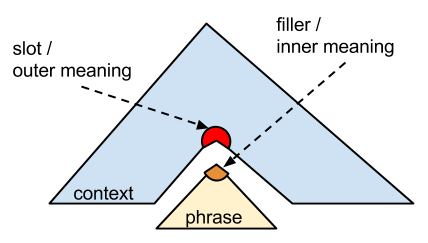
\includegraphics[scale=0.5]{Inner_outer.png}
	\caption{If there is a strong correlation between outer meaning and inner meaning, a dynamic
	binding occurs.}
	\label{figure inner outer}
\end{figure}



\subsection{Potential Extensions / Future Work}
\label{subsection future work}

Our new architecture IORNN has many potential extensions, some of which are promising to improve 
the performance in those two tasks presented above, other could lead to important applications. 

\paragraph{At lexicon level} In Subsection~\ref{subsection wsc}, we 
have seen multi-prototype approaches are promising for computing word meaning in 
context. Certainly, we can combine these approaches with our framework IORNN at the 
lexical level in order to disambiguate word senses. 

\paragraph{At syntax level} IORNN only uses parse trees without grammatical categories. However, 
\newcite{hermann2013role} empirically show the important role of syntax in vector space models of 
compositional semantics. It turns out that it is also easy to extend IORNN in the same way, 
i.e. using CCG and different parameter sets for different 
grammatical rules and grammatical types. Thanks to some degree of similarity between IORNN and 
RAE, we expect that this extension helps IORNN improve its capacity in capturing compositionality.

\paragraph{At discourse level} In this paper, we propose IORNN as an architecture 
processing individual sentences; therefore, the outer meaning at the root node is alway a 
null-context outer meaning vector (i.e., $\mathbf{o}_{root} = \mathbf{o}_{\emptyset}$).
Beyond that, we can extend IORNN to make use of discourse context.
Figure~\ref{figure dciornn} illustrates how to connect inner and outer meanings 
of sentences in a discourse. Intuitively, the outer meaning of a sentence is 
the function of the inner meanings of its neighbours.

\begin{figure}[h!]
	\center
	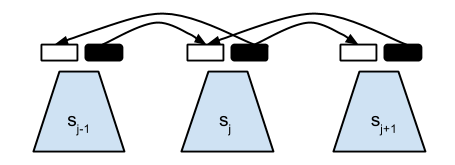
\includegraphics[scale=0.5]{DC-IO-RNN.png}
	\caption{IORNN with discourse context. 
	Black rectangles correspond to inner meanings, 
	white rectangles correspond to outer meanings.}
	\label{figure dciornn}
\end{figure}


%%%%%%%%%%%%%%%%%%%%%%%%%%%%%%%%%%%%%%%%%%%

\section{Conclusion}
\label{section conclusion}

In this paper, we presented a unified framework, namely Inside Outside Recursive
Neural Network, that tackles both compositional semantics and meaning in context. 
Similar to RNN, IORNN uses recursive network architecture to construct 
phrase representations, but different in that it also constructs context representations and 
is trained in a very different manner. The training, based on our new hypothesis, 
only needs contexts of words and thus avoids the sparsity of data, unlike the works of 
\newcite{baroni_frege_2012}, \newcite{grefenstette_multi-step_2013}.




\bibliographystyle{apalike}
\bibliography{ref}

\end{document}
